\documentclass[11pt, oneside]{article}    % use "amsart" instead of "article" for AMSLaTeX format

\usepackage[letterpaper,margin=1in]{geometry}
\usepackage{booktabs}
\usepackage[numbers]{natbib}
\usepackage{hyperref}
\usepackage{enumitem}
\usepackage{float}
\usepackage{caption}
\usepackage{subcaption}
\usepackage{graphicx}
\usepackage{amssymb}

\title{CS780 Capstone Project: \\
OBELIX: the Warehouse Robot
}

\author{
    FirstName $<$Middle Name if any$>$ LastName  \\ 
    roll no.\\
    {\tt arpity22@iitk.ac.in}\\
    {Indian Institute of Technology Kanpur (IIT Kanpur)}
}

\date{}

\begin{document}

\maketitle

\begin{abstract}
OBELIX is a partially observable warehouse-robot task where the agent must locate a box using sparse binary sensors, attach to it, and push it to the boundary while avoiding repeated ``stuck'' events and wall obstacles. We implemented a progression of reinforcement learning agents: Double/Dueling DQN with prioritized experience replay, recurrent Q-learning variants to handle blinking/moving targets, and several PPO stabilizations. Our final submission focuses on a recurrent actor-critic trained with PPO plus auxiliary intrinsic learning (random network distillation) and deterministic search/stuck-recovery heuristics for robustness. We summarize training dynamics and local evaluation evidence across the three difficulty levels.
\end{abstract}

\section{Competition Result}
\textbf{Codabench Username:} \textbf{a\_220206} \\
\textbf{Final leaderboard rank (Test Phase):} \textbf{45} \\
\textbf{Leaderboard rank -- Level 1 (static):} \textbf{36} \\
\textbf{Leaderboard rank -- Level 2 (blinking):} \textbf{71} \\
\textbf{Leaderboard rank -- Level 3 (moving + blinking):} \textbf{70} \\

The repository contains 29 locally packaged ``submission'' directories used during development (many also contain a ready-to-upload \texttt{submission.zip}). Table~\ref{tab:submission-counts} summarizes them by method family.

\begin{table}[H]
\centering
\caption{Local submission packages created during development (repository evidence).}
\label{tab:submission-counts}
\begin{tabular}{lrl}
\toprule
Method family & Count & Examples (directories) \\
\midrule
D3QN-PER (dueling+double+PER) & 11 & \texttt{submission\_001}, \texttt{\_002\_no\_wall}, \texttt{phase4\_final} \\
PPO variants & 7 & \texttt{submission\_ppo\_test}, \texttt{\_adaptive\_v1}, \texttt{\_adv\_final} \\
RAPTOR-PPO variants & 5 & \texttt{submission\_raptor\_ppo} (\& \texttt{\_ppo1--\_ppo4}) \\
Recurrent DQN variants (ADRQN/RD3QN) & 3 & \texttt{submission\_adrqn.py}, \texttt{submission\_rd3qn} \\
World model (POMDP) & 1 & \texttt{submission\_worldmodel\_pomdp1} \\
Debug/other & 2 & \texttt{submission\_debug\_tmp}, \texttt{submission\_improved\_lstm} \\
\bottomrule
\end{tabular}
\end{table}

\section{Introduction and Problem Description}
OBELIX is a simulated warehouse-robot domain inspired by the classic behavior-based robotics setting by Mahadevan et. al \citep{mahadevan1991automatic}. The agent controls a differential-drive robot using a small discrete action set: turn left/right by $22.5^{\circ}$ or $45^{\circ}$, or move forward. At each step the robot receives an 18-dimensional binary observation summarizing local proximity sensing (sonar bits), an IR cue, and a "stuck"``stuck'' flag. The goal is to locate the grey box, attach to it, and then push the attached box until it touches the arena boundary, which terminates the episode with a large terminal reward.

The environment exposes three difficulty modes. Level~1 (difficulty 0 in code) uses a static box. Level~2 (difficulty 2) makes the box intermittently visible (blinking), which creates partial observability because the same local sensor readings can correspond to multiple latent box positions. Level~3 (difficulty 3) additionally moves the box while blinking, introducing non-stationarity and requiring both memory and robust interception behavior. An additional robustness axis enables wall obstacles, which creates dead-ends and increases the probability of repetitive collision loops.

Overall, this is a POMDP: the current observation is insufficient to fully infer the box pose, the robot pose relative to obstacles, or whether the box has recently blinked out of view. The high-level objective in this project was to maximize mean cumulative reward under the Codabench evaluation protocol (multiple random seeds, fixed horizon) across all three difficulties while remaining robust to wall obstacles.

\section{Approach and Model Evolution}
We followed an iterative ``baseline $\rightarrow$ stabilize $\rightarrow$ add memory $\rightarrow$ improve exploration'' workflow. The main bottlenecks observed early were (i) sparse successful trajectories (attach+push to boundary), (ii) severe penalties from the stuck flag, and (iii) partial observability at higher levels (blinking and moving targets). This led to two broad families of solutions: value-based replay methods that can reuse rare successes, and on-policy actor-critic methods that can incorporate recurrent memory and entropy-based exploration.

\subsection{Value-based baselines: Double/Dueling DQN with PER}
Our initial agents used Double DQN \citep{vanhasselt2016double} to reduce overestimation, and then moved to a dueling architecture \citep{wang2016dueling} with prioritized experience replay (PER) \citep{schaul2016per}. The dueling split helps learn state value even when actions are not immediately differentiating, while PER increases the sampling rate of high TD-error transitions (often rare near-success or recovery events). For evaluation, we used greedy action selection with a small ``action smoothing'' rule to reduce oscillations when the top Q-values are nearly tied.

These agents operate directly on the raw 18-bit observation vector, which is attractive for simplicity but limits the ability to infer latent box motion or handle blinking without history.

\subsection{POMDP extensions: recurrent value learning and auxiliary belief}
To address blinking/moving targets, we explored recurrent value learning (ADRQN/RD3QN-style) by augmenting the Q-network with an LSTM/GRU over recent observations and actions. In addition, one variant introduced a simple spatial ``belief'' map feature to stabilize navigation under partial observability. The recurrent models improved qualitative tracking in Level~2/3, but were sensitive to hidden-state reset behavior and to train--test mismatches in how episode boundaries are detected.

\subsection{On-policy actor-critic: PPO variants and stabilizations}
We implemented PPO \citep{schulman2017ppo} with generalized advantage estimation (GAE) \citep{schulman2016gae} and iterated through several stabilizations: timeout-aware bootstrapping, entropy schedules to balance exploration/exploitation, and optional recurrent policies. PPO was especially convenient for experimenting with reward-shaping knobs (e.g., encouraging forward motion when front sensors are active) and for controlling exploration through an entropy bonus.

\subsection{Final model: recurrent PPO with intrinsic learning (RAPTOR-PPO)}
Our final submission is a recurrent actor-critic trained with PPO and augmented with intrinsic motivation via random network distillation (RND) \citep{burda2019rnd} and an auxiliary next-observation prediction head. The motivation is that Level~2/3 require persistent exploration under intermittent observability, and intrinsic novelty rewards help discover attach/push behaviors more reliably.

\paragraph{Architecture and state representation.}
The policy consumes an augmented feature vector built from the raw observation $o_t\in\mathbb{R}^{18}$, a first-difference feature $\Delta o_t=o_t-o_{t-1}$, a one-hot encoding of the previous action, and two small scalars that summarize ``time since last seeing the target'' and normalized episode progress (43 dimensions total). This is passed through an MLP encoder and a GRU memory. The GRU hidden state feeds a policy head (5-way logits) and a value head. Figure~\ref{fig:arch} shows a schematic.

\begin{figure}[H]
\centering
\fbox{\begin{minipage}{0.92\linewidth}
\centering
Raw sensors $o_t$ (18D) $\rightarrow$ feature augmentation (delta, last-action one-hot, timers) $\rightarrow$ MLP encoder $\rightarrow$ GRU memory $\rightarrow$ \{policy logits, value\}.
\end{minipage}}
\caption{Schematic of the final recurrent actor-critic (RAPTOR-PPO) used for evaluation.}
\label{fig:arch}
\end{figure}

\paragraph{Exploration and shaping.}
PPO exploration is controlled primarily through an entropy bonus. For the intrinsic component, an RND predictor provides a novelty signal that is annealed down over training so that the final policy relies on extrinsic reward. We also included deterministic ``search'' and ``stuck recovery'' heuristics in the action selection logic (e.g., turn--turn--forward cycles when the stuck flag is raised) to increase robustness with walls; this mirrors the behavior-based decomposition spirit of \citep{mahadevan1991automatic} even though the final policy is trained end-to-end.

\section{Experiments and Implementation Details}
All training and evaluation code is implemented in Python. The OBELIX simulator is in \texttt{obelix.py} (OpenCV-based dynamics and sensing). For reproducibility we used fixed evaluation settings consistent with the provided evaluator: horizon 1000 steps, wall obstacles enabled for robustness tests, and difficulty levels $\{0,2,3\}$. During training, we checkpointed periodically and selected submission checkpoints based on deterministic evaluation runs.

Most experiments were run CPU-only (matching the Codabench inference constraint). Training budgets varied by variant: value-based runs typically used 1000--4000 episodes with 1000 max steps, while PPO variants used 1--2 million environment steps with parallel rollout workers. Based on the stored training logs, end-to-end wall-obstacle runs ranged from roughly $\sim$33 minutes (e.g., \texttt{submission\_phase4\_final}) to $\sim$158 minutes (e.g., \texttt{submission\_001}) depending on algorithm and data-collection parallelism.

We also explored curriculum-style training (\texttt{train\_curriculum.py}) that progressively increased difficulty and/or reduced shaping as performance improved. While this improved early learning stability, the final strategy prioritized robustness on the hardest settings (Level~3 with walls) via recurrent policies and explicit stuck-recovery behavior.

Table~\ref{tab:hparams} summarizes representative hyperparameters for the major agent families. For value-based methods, we used an Adam optimizer, replay buffers up to $10^5$ transitions, and periodic target-network synchronization. For PPO, we used GAE, mini-batch SGD over rollout data, and (in the recurrent variants) truncated backpropagation through time over short sequences.

\begin{table}[H]
\centering
\caption{Representative hyperparameters used for major model variants (defaults as implemented in the training scripts).}
\label{tab:hparams}
\begin{tabular}{lcccc}
\toprule
Variant & $\gamma$ & LR & Batch/rollout & Notable settings \\
\midrule
D3QN-PER \citep{schaul2016per,wang2016dueling,vanhasselt2016double} & 0.99 & $5\times10^{-4}$ & 256 & replay $10^5$, PER $\alpha=0.6$, $\beta:0.4\rightarrow1$ \\
PPO baseline \citep{schulman2017ppo} & 0.99 & $3\times10^{-4}$ & 2048/256 & 10 epochs, clip $0.2$, entropy bonus $\approx 10^{-2}$ \\
RAPTOR-PPO (final) & 0.995 & $3\times10^{-4}$ & 512 horizon & GRU(192), RND intrinsic coef annealed to 0 \\
World-model (exploratory) \citep{hafner2020dreamer} & 0.995 & $\sim 2\times10^{-4}$ & seq 32 / 64 & latent model + imagination rollouts (not final) \\
\bottomrule
\end{tabular}
\end{table}

\paragraph{Local evaluation.}
We used \texttt{evaluate.py} to compute mean and standard deviation of episodic scores over multiple random seeds, appending results to \texttt{leaderboard.csv}. To approximate the Codabench protocol, we also used \texttt{evaluate\_on\_codabench.py}, which runs 10 episodes per difficulty with wall obstacles enabled and reports mean/std scores per level.

\section{Results}
This repository contains rich development evidence (training logs, diagnostic plots, and local evaluation summaries). However, official Codabench ranks are not stored in the repository, so the ``Test Phase'' leaderboard fields in Section~1 must be filled from the Codabench page.

\subsection{Local leaderboard snapshots}
The file \texttt{leaderboard.csv} stores local evaluation rows (mean/std scores over multiple runs). An example snapshot for the provided template agent shows strongly negative mean scores at high difficulty with walls, indicating that avoiding repeated stuck penalties is critical.

\subsection{Training-log evidence across phases}
Several development submissions include \texttt{training\_log.txt} with aggregate returns and success rates. Table~\ref{tab:train-logs} highlights representative runs.

\begin{table}[H]
\centering
\caption{Representative training-log summaries from development submissions (success = fraction of episodes reaching the terminal attach+boundary condition as logged by the trainer).}
\label{tab:train-logs}
\begin{tabular}{lrrrr}
\toprule
Submission & Episodes & Mean return & Success rate & Best success \\
\midrule
\texttt{submission\_001} & 3000 & -108260 & 16\% & 32\% \\
\texttt{submission\_002\_no\_wall} & 2000 & -1185 & 0\% & 24\% \\
\texttt{submission\_FIXED\_shaped} & 4000 & -30453 & 7\% & 30\% \\
\texttt{submission\_phase2\_medium} & 2000 & -116957 & 16\% & 17\% \\
\texttt{submission\_phase4\_final} & 1000 & -27510 & 7\% & 23\% \\
\bottomrule
\end{tabular}
\end{table}

\subsection{Learning curves and diagnostics}
Figure~\ref{fig:learning-curves} shows two representative training summaries from D3QN-PER development runs. The plots show high variance in episodic returns and sparse success events, consistent with a task dominated by step penalties and occasional large terminal rewards.

\begin{figure}[H]
\centering
\begin{subfigure}[b]{0.49\textwidth}
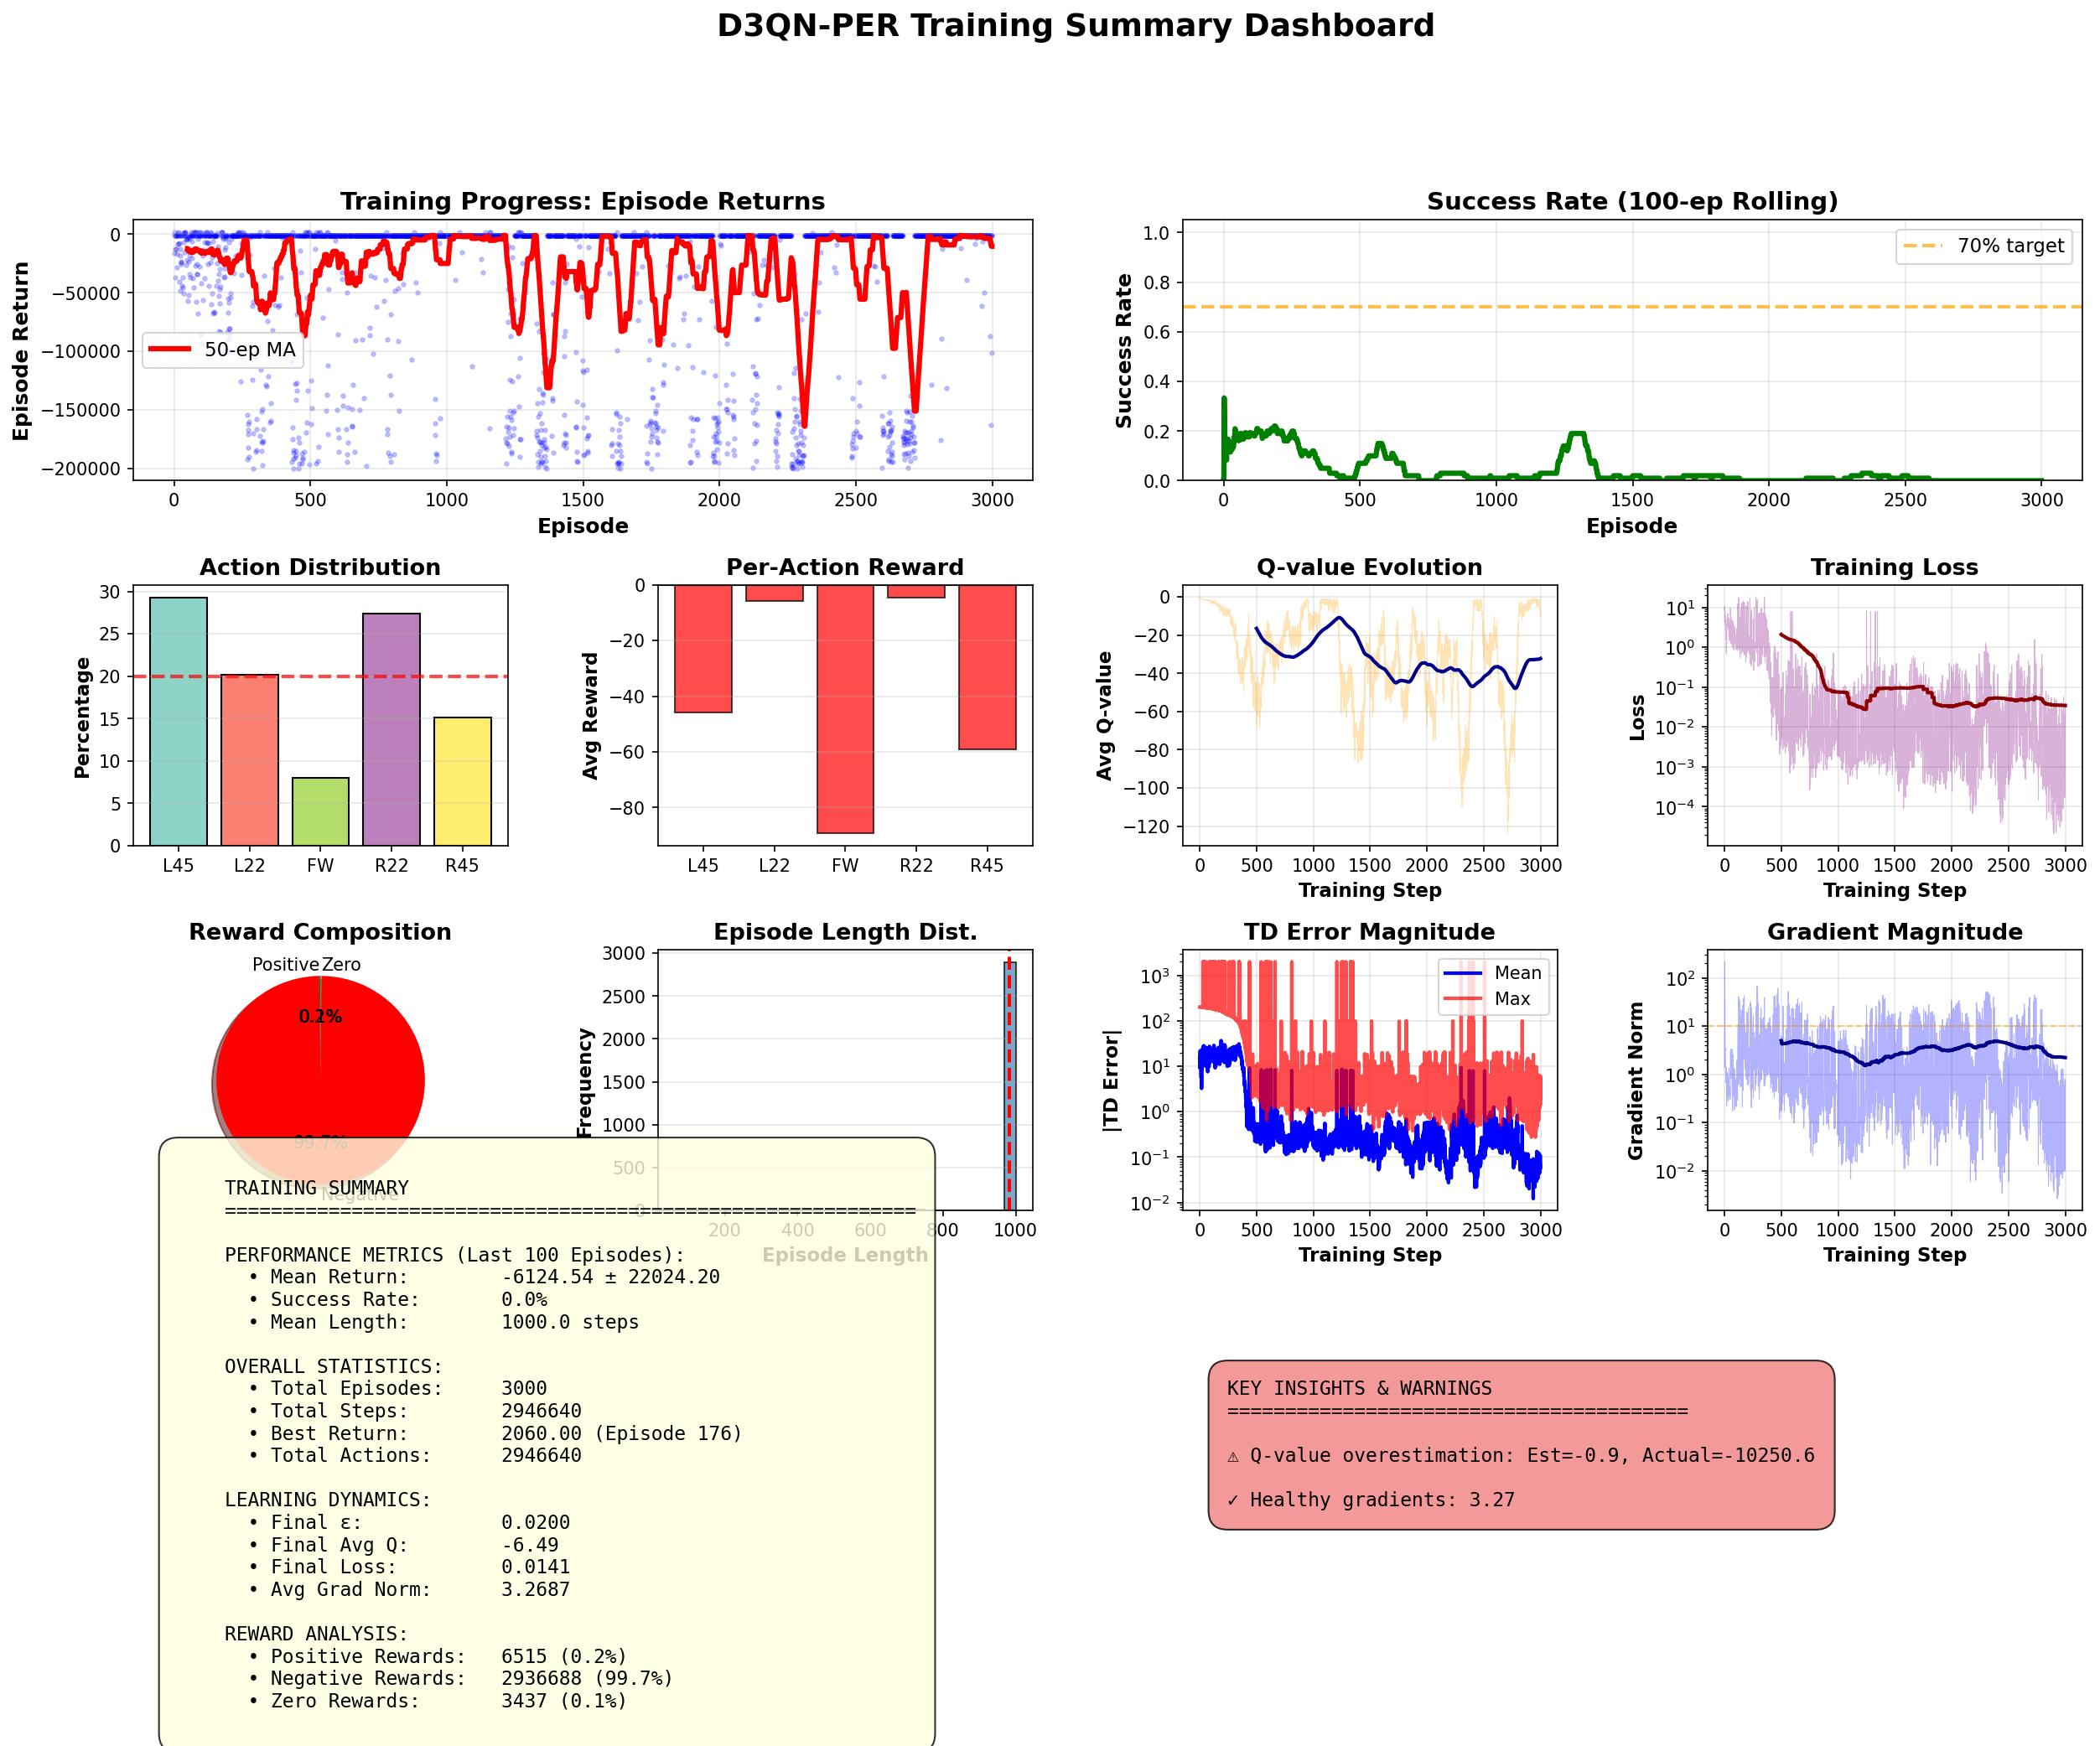
\includegraphics[width=\textwidth]{../submission_001_no_wall/training_summary.png}
\caption{D3QN-PER (no wall obstacles).}
\end{subfigure}
\hfill
\begin{subfigure}[b]{0.49\textwidth}
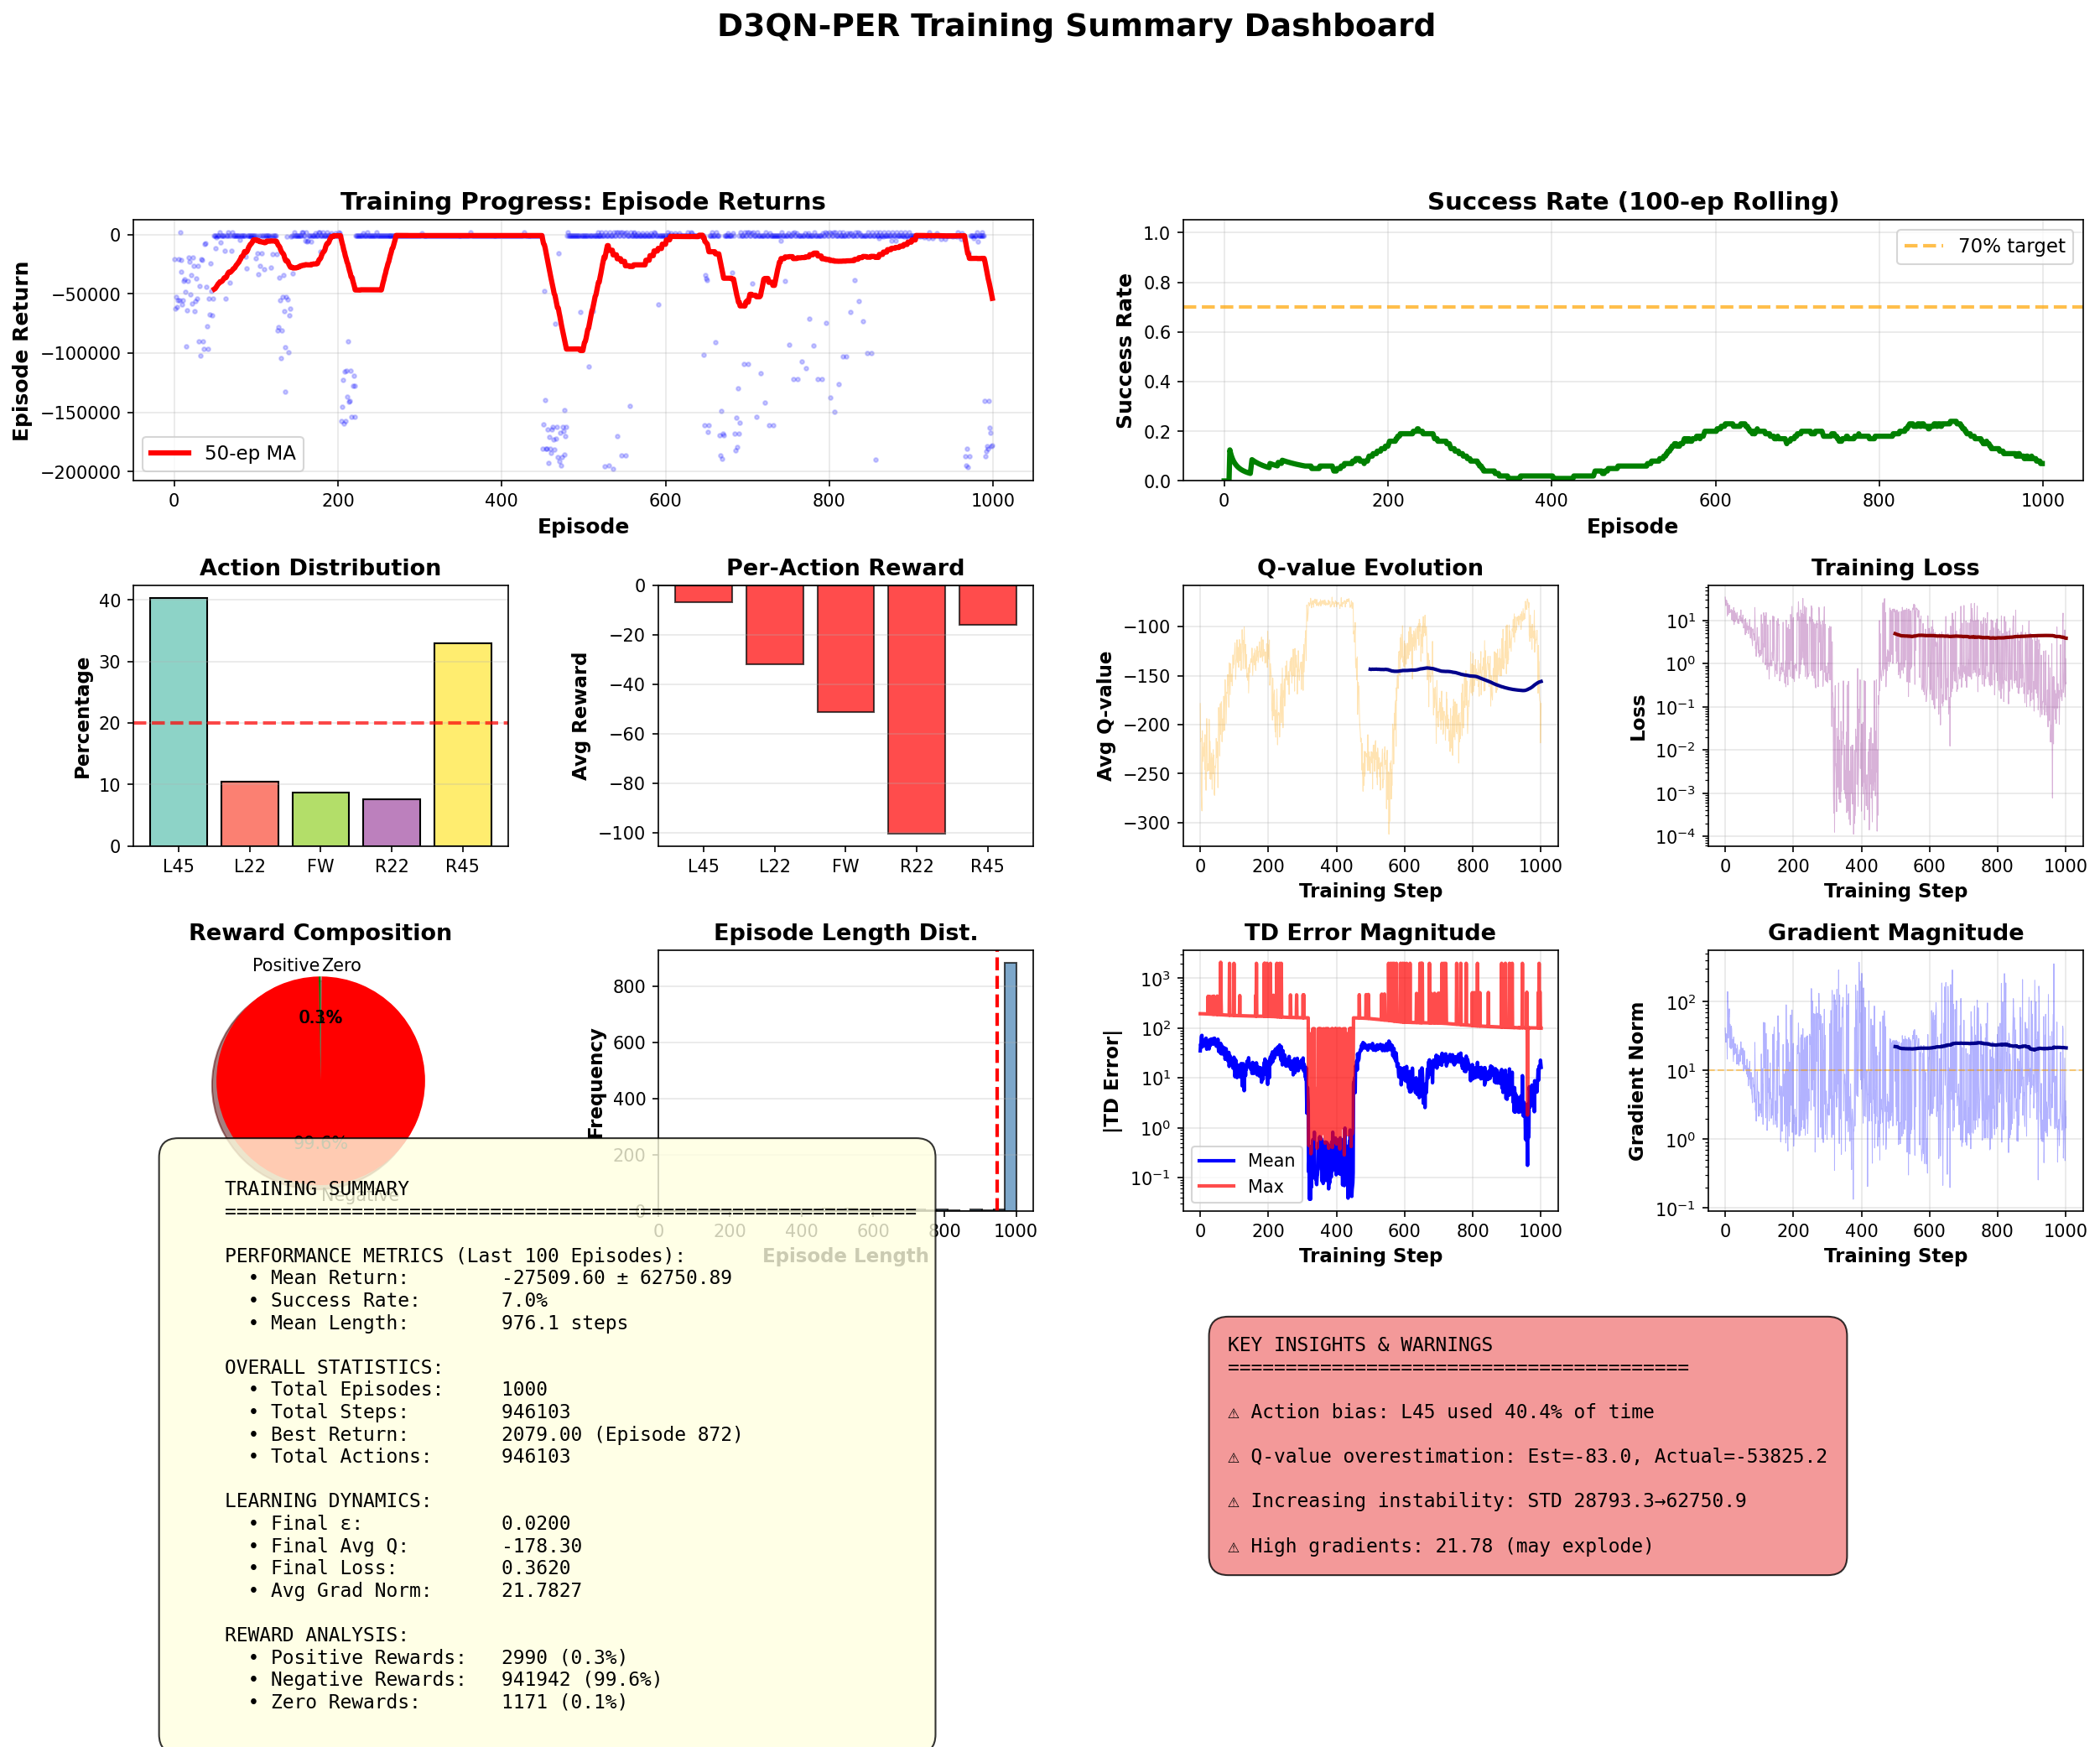
\includegraphics[width=\textwidth]{../submission_phase4_final/training_summary.png}
\caption{D3QN-PER (final shaped phase).}
\end{subfigure}
\caption{Representative learning curves from development submissions (generated by training scripts).}
\label{fig:learning-curves}
\end{figure}

\paragraph{Which model performed best and why?}
In our development workflow, the strongest improvements came from (i) stabilizing learning dynamics (target networks / PPO clipping), (ii) adding memory for blinking/moving targets (recurrent policies), and (iii) enforcing robust recovery behavior when the stuck flag becomes active (crucial with wall obstacles). Intrinsic motivation helped exploration early, but required annealing so that the final behavior optimizes extrinsic success.

\section{Error Analysis and Discussion}
\paragraph{Failure modes by difficulty.}
Even in Level~1, failures occur when the robot enters local limit cycles: repeated turning in place, ``bouncing'' off walls, or approaching the box at an angle that causes immediate stuck penalties. In Level~2, blinking introduces false negatives: the agent can lose track of the box after it disappears, making greedy policies overreact to short-term sensor noise. Level~3 adds box motion, which creates interception errors and increases the likelihood of overshooting or pushing the box into awkward corners.

\paragraph{Walls and stuck dynamics.}
With wall obstacles enabled, the dominant failure mode is getting trapped in corners or narrow passages and repeatedly triggering the stuck flag (large negative penalties). Robust policies require an explicit recovery behavior (e.g., alternating turns and forward motion) and should avoid committing to tight turns when front sensors indicate imminent collision.

\paragraph{Evaluation mismatches.}
One subtle issue we encountered is that some training/evaluation utilities infer ``success'' using a reward threshold, while the environment applies per-step penalties even in successful episodes. This can underreport success in logs and can mis-rank checkpoints. A more reliable definition is to derive success from the terminal condition (attached box reaching the boundary) rather than from reward magnitude.

\paragraph{What we would improve with more time.}
Two clear directions are (i) making POMDP handling more principled (e.g., better recurrent state management or latent-state models \citep{hafner2020dreamer}), and (ii) improving wall-robust navigation by explicitly learning a short-horizon obstacle-avoidance controller that can be composed with the box-seeking/pushing behavior.

\section{Conclusion}
We explored a broad design space for OBELIX, progressing from replay-based value learning to recurrent actor-critic methods with intrinsic motivation. The main lesson is that partial observability and ``stuck'' dynamics dominate performance: memory helps track intermittent targets, but robustness ultimately depends on reliable recovery behaviors and evaluation discipline (consistent success definitions and checkpoint selection). Future work could incorporate stronger latent-state world models, richer observations, and more realistic physics to reduce the gap between simulation strategies and real-robot robustness.

\section*{LLM Usage Declaration}
\begin{itemize}
\item \textbf{Which LLM was used?} GitHub Copilot Chat (GPT-5.2) was used to help structure the report and to summarize code/experiment artifacts in the repository.

\item \textbf{In which part was the LLM used, and how did it help?}

\begin{tabular}{l|l|l}
\toprule
Part & Used LLM? (Yes/No) & Purpose of Using LLM \\
\midrule
Understanding concepts & Yes & Clarifying PPO/DQN variants and POMDP framing \\
Ideation / brainstorming & Yes & Organizing the approach-evolution narrative \\
Debugging small code snippets & Yes & Minor checks and small refactors during development \\
Plotting / visualization code & No & (Plots were generated by existing training scripts) \\
Grammar / writing style & Yes & Editing for clarity and concision \\
Report structure / section ideas & Yes & Mapping repository evidence into the template \\
Other (specify) & No &  \\
\bottomrule
\end{tabular}

\item \textbf{Other sources used (besides the LLM and slides).} We referenced standard RL papers for DQN/PPO/PER/RND and the original OBELIX paper \citep{mahadevan1991automatic}. We also consulted OpenCV documentation as needed for environment rendering/debugging.

\item \textbf{Own contribution.} We implemented multiple agents and training pipelines in PyTorch, designed and tuned reward shaping/exploration schedules, ran systematic experiments across difficulty levels (including wall robustness), and performed checkpoint selection and error analysis based on local evaluator logs and diagnostic plots.
\end{itemize}

\vspace{2cm}

\bibliographystyle{ieeetr}
\bibliography{references}

% Optional appendix (only if explicitly allowed by TAs)
% \newpage
% \appendix
% \section{Additional Plots / Ablations}

\end{document}